% Created by tikzDevice version 0.12.6 on 2025-04-24 16:39:58
% !TEX encoding = UTF-8 Unicode
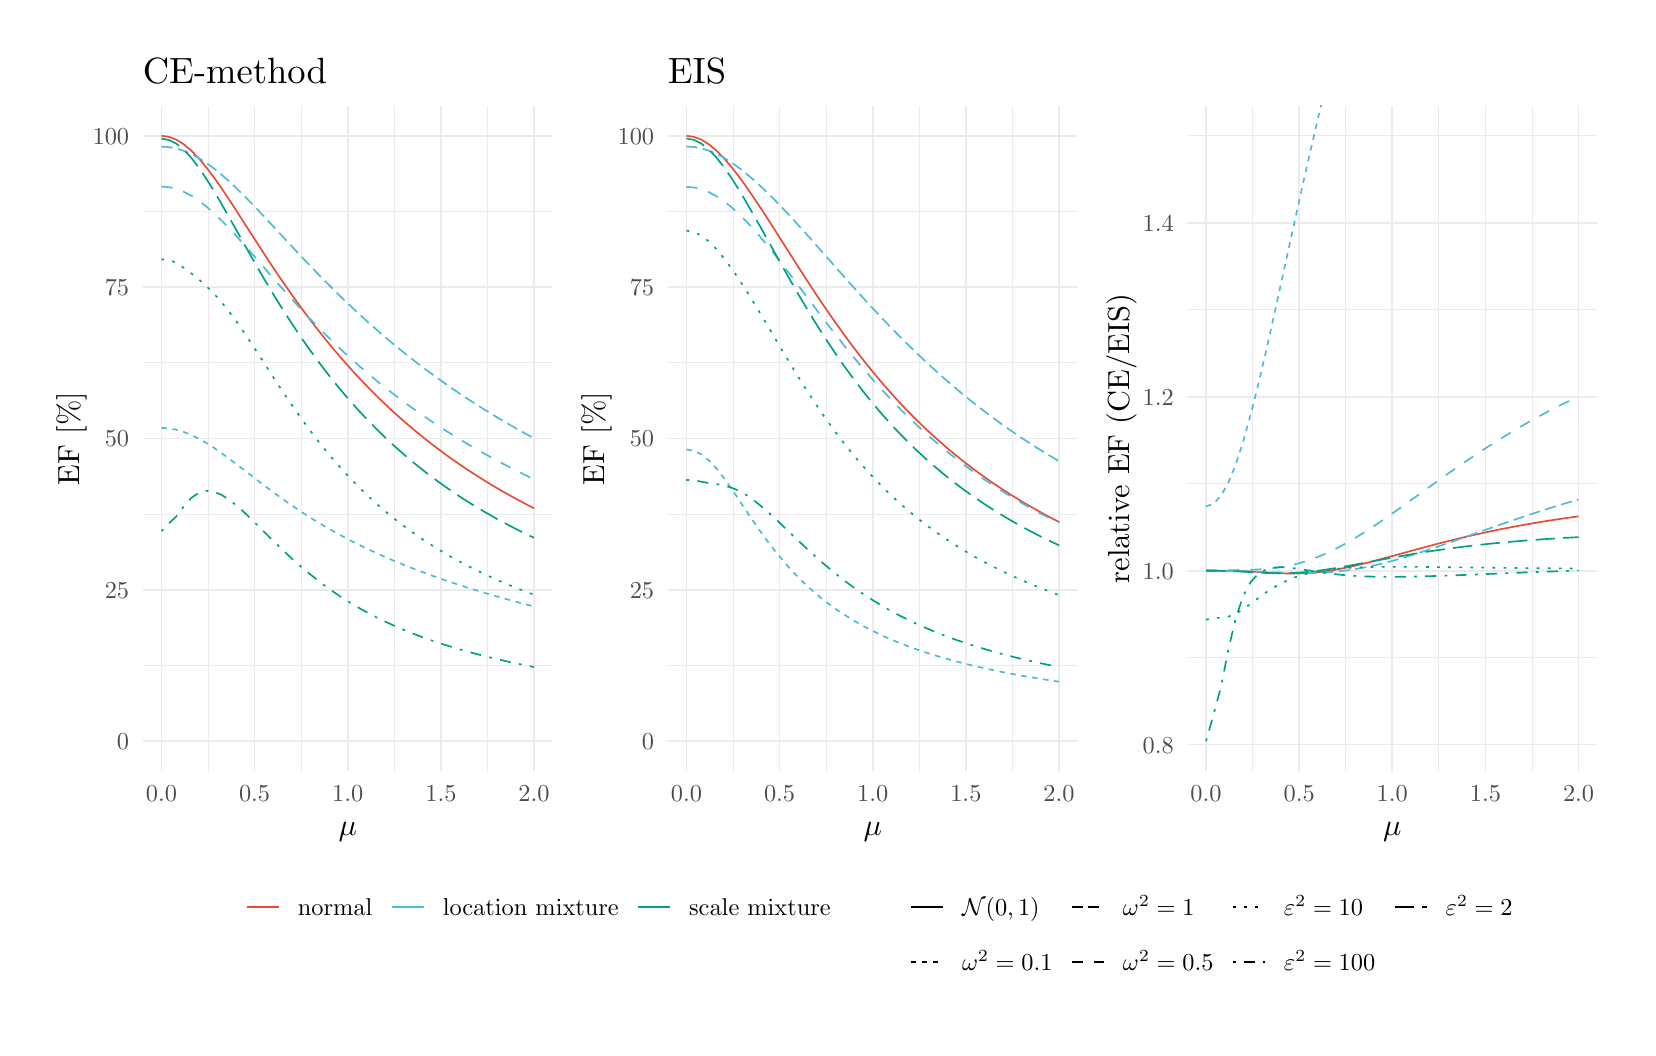
\begin{tikzpicture}[x=1pt,y=1pt]
\definecolor{fillColor}{RGB}{255,255,255}
\path[use as bounding box,fill=fillColor,fill opacity=0.00] (0,0) rectangle (578.16,361.35);
\begin{scope}
\path[clip] ( 41.61, 92.59) rectangle (189.71,333.19);
\definecolor{drawColor}{gray}{0.92}

\path[draw=drawColor,line width= 0.3pt,line join=round] ( 41.61,130.87) --
	(189.71,130.87);

\path[draw=drawColor,line width= 0.3pt,line join=round] ( 41.61,185.55) --
	(189.71,185.55);

\path[draw=drawColor,line width= 0.3pt,line join=round] ( 41.61,240.23) --
	(189.71,240.23);

\path[draw=drawColor,line width= 0.3pt,line join=round] ( 41.61,294.92) --
	(189.71,294.92);

\path[draw=drawColor,line width= 0.3pt,line join=round] ( 65.17, 92.59) --
	( 65.17,333.19);

\path[draw=drawColor,line width= 0.3pt,line join=round] ( 98.83, 92.59) --
	( 98.83,333.19);

\path[draw=drawColor,line width= 0.3pt,line join=round] (132.49, 92.59) --
	(132.49,333.19);

\path[draw=drawColor,line width= 0.3pt,line join=round] (166.14, 92.59) --
	(166.14,333.19);

\path[draw=drawColor,line width= 0.6pt,line join=round] ( 41.61,103.53) --
	(189.71,103.53);

\path[draw=drawColor,line width= 0.6pt,line join=round] ( 41.61,158.21) --
	(189.71,158.21);

\path[draw=drawColor,line width= 0.6pt,line join=round] ( 41.61,212.89) --
	(189.71,212.89);

\path[draw=drawColor,line width= 0.6pt,line join=round] ( 41.61,267.57) --
	(189.71,267.57);

\path[draw=drawColor,line width= 0.6pt,line join=round] ( 41.61,322.26) --
	(189.71,322.26);

\path[draw=drawColor,line width= 0.6pt,line join=round] ( 48.34, 92.59) --
	( 48.34,333.19);

\path[draw=drawColor,line width= 0.6pt,line join=round] ( 82.00, 92.59) --
	( 82.00,333.19);

\path[draw=drawColor,line width= 0.6pt,line join=round] (115.66, 92.59) --
	(115.66,333.19);

\path[draw=drawColor,line width= 0.6pt,line join=round] (149.32, 92.59) --
	(149.32,333.19);

\path[draw=drawColor,line width= 0.6pt,line join=round] (182.97, 92.59) --
	(182.97,333.19);
\definecolor{drawColor}{RGB}{230,75,53}

\path[draw=drawColor,line width= 0.6pt,line join=round] ( 48.34,322.26) --
	( 51.04,321.91) --
	( 53.73,320.87) --
	( 56.42,319.19) --
	( 59.11,316.93) --
	( 61.81,314.15) --
	( 64.50,310.94) --
	( 67.19,307.38) --
	( 69.88,303.57) --
	( 72.58,299.56) --
	( 75.27,295.44) --
	( 77.96,291.25) --
	( 80.65,287.04) --
	( 83.35,282.85) --
	( 86.04,278.70) --
	( 88.73,274.62) --
	( 91.42,270.62) --
	( 94.12,266.72) --
	( 96.81,262.92) --
	( 99.50,259.22) --
	(102.20,255.63) --
	(104.89,252.14) --
	(107.58,248.76) --
	(110.27,245.49) --
	(112.97,242.32) --
	(115.66,239.26) --
	(118.35,236.29) --
	(121.04,233.42) --
	(123.74,230.64) --
	(126.43,227.96) --
	(129.12,225.36) --
	(131.81,222.84) --
	(134.51,220.41) --
	(137.20,218.06) --
	(139.89,215.78) --
	(142.58,213.58) --
	(145.28,211.44) --
	(147.97,209.38) --
	(150.66,207.38) --
	(153.35,205.44) --
	(156.05,203.57) --
	(158.74,201.75) --
	(161.43,199.99) --
	(164.13,198.28) --
	(166.82,196.62) --
	(169.51,195.02) --
	(172.20,193.46) --
	(174.90,191.95) --
	(177.59,190.48) --
	(180.28,189.06) --
	(182.97,187.68);
\definecolor{drawColor}{RGB}{77,187,213}

\path[draw=drawColor,line width= 0.6pt,dash pattern=on 2pt off 2pt ,line join=round] ( 48.34,216.73) --
	( 51.04,216.56) --
	( 53.73,216.07) --
	( 56.42,215.28) --
	( 59.11,214.20) --
	( 61.81,212.87) --
	( 64.50,211.33) --
	( 67.19,209.60) --
	( 69.88,207.74) --
	( 72.58,205.78) --
	( 75.27,203.75) --
	( 77.96,201.69) --
	( 80.65,199.61) --
	( 83.35,197.54) --
	( 86.04,195.50) --
	( 88.73,193.49) --
	( 91.42,191.53) --
	( 94.12,189.63) --
	( 96.81,187.79) --
	( 99.50,186.00) --
	(102.20,184.28) --
	(104.89,182.62) --
	(107.58,181.02) --
	(110.27,179.48) --
	(112.97,177.99) --
	(115.66,176.56) --
	(118.35,175.18) --
	(121.04,173.84) --
	(123.74,172.55) --
	(126.43,171.31) --
	(129.12,170.11) --
	(131.81,168.94) --
	(134.51,167.81) --
	(137.20,166.72) --
	(139.89,165.66) --
	(142.58,164.64) --
	(145.28,163.64) --
	(147.97,162.67) --
	(150.66,161.73) --
	(153.35,160.81) --
	(156.05,159.92) --
	(158.74,159.06) --
	(161.43,158.22) --
	(164.13,157.40) --
	(166.82,156.60) --
	(169.51,155.82) --
	(172.20,155.06) --
	(174.90,154.32) --
	(177.59,153.60) --
	(180.28,152.89) --
	(182.97,152.21);

\path[draw=drawColor,line width= 0.6pt,dash pattern=on 4pt off 2pt ,line join=round] ( 48.34,318.36) --
	( 51.04,318.19) --
	( 53.73,317.68) --
	( 56.42,316.84) --
	( 59.11,315.68) --
	( 61.81,314.23) --
	( 64.50,312.51) --
	( 67.19,310.55) --
	( 69.88,308.37) --
	( 72.58,306.01) --
	( 75.27,303.50) --
	( 77.96,300.86) --
	( 80.65,298.12) --
	( 83.35,295.31) --
	( 86.04,292.45) --
	( 88.73,289.56) --
	( 91.42,286.66) --
	( 94.12,283.75) --
	( 96.81,280.87) --
	( 99.50,278.00) --
	(102.20,275.17) --
	(104.89,272.38) --
	(107.58,269.64) --
	(110.27,266.94) --
	(112.97,264.30) --
	(115.66,261.71) --
	(118.35,259.17) --
	(121.04,256.69) --
	(123.74,254.26) --
	(126.43,251.89) --
	(129.12,249.58) --
	(131.81,247.31) --
	(134.51,245.10) --
	(137.20,242.94) --
	(139.89,240.84) --
	(142.58,238.78) --
	(145.28,236.76) --
	(147.97,234.80) --
	(150.66,232.88) --
	(153.35,231.00) --
	(156.05,229.17) --
	(158.74,227.38) --
	(161.43,225.63) --
	(164.13,223.92) --
	(166.82,222.25) --
	(169.51,220.62) --
	(172.20,219.02) --
	(174.90,217.46) --
	(177.59,215.93) --
	(180.28,214.43) --
	(182.97,212.97);

\path[draw=drawColor,line width= 0.6pt,dash pattern=on 4pt off 4pt ,line join=round] ( 48.34,303.92) --
	( 51.04,303.71) --
	( 53.73,303.07) --
	( 56.42,302.03) --
	( 59.11,300.61) --
	( 61.81,298.84) --
	( 64.50,296.77) --
	( 67.19,294.42) --
	( 69.88,291.85) --
	( 72.58,289.10) --
	( 75.27,286.20) --
	( 77.96,283.21) --
	( 80.65,280.15) --
	( 83.35,277.05) --
	( 86.04,273.94) --
	( 88.73,270.84) --
	( 91.42,267.76) --
	( 94.12,264.73) --
	( 96.81,261.76) --
	( 99.50,258.84) --
	(102.20,255.99) --
	(104.89,253.21) --
	(107.58,250.49) --
	(110.27,247.86) --
	(112.97,245.29) --
	(115.66,242.80) --
	(118.35,240.37) --
	(121.04,238.02) --
	(123.74,235.73) --
	(126.43,233.50) --
	(129.12,231.34) --
	(131.81,229.24) --
	(134.51,227.19) --
	(137.20,225.20) --
	(139.89,223.26) --
	(142.58,221.38) --
	(145.28,219.54) --
	(147.97,217.75) --
	(150.66,216.01) --
	(153.35,214.31) --
	(156.05,212.66) --
	(158.74,211.04) --
	(161.43,209.47) --
	(164.13,207.93) --
	(166.82,206.43) --
	(169.51,204.97) --
	(172.20,203.54) --
	(174.90,202.15) --
	(177.59,200.79) --
	(180.28,199.46) --
	(182.97,198.15);
\definecolor{drawColor}{RGB}{0,160,135}

\path[draw=drawColor,line width= 0.6pt,dash pattern=on 1pt off 3pt ,line join=round] ( 48.34,277.59) --
	( 51.04,277.55) --
	( 53.73,276.30) --
	( 56.42,274.57) --
	( 59.11,272.59) --
	( 61.81,270.43) --
	( 64.50,268.04) --
	( 67.19,265.37) --
	( 69.88,262.36) --
	( 72.58,259.03) --
	( 75.27,255.40) --
	( 77.96,251.55) --
	( 80.65,247.52) --
	( 83.35,243.40) --
	( 86.04,239.24) --
	( 88.73,235.08) --
	( 91.42,230.98) --
	( 94.12,226.96) --
	( 96.81,223.05) --
	( 99.50,219.26) --
	(102.20,215.60) --
	(104.89,212.09) --
	(107.58,208.72) --
	(110.27,205.50) --
	(112.97,202.42) --
	(115.66,199.47) --
	(118.35,196.66) --
	(121.04,193.99) --
	(123.74,191.43) --
	(126.43,188.99) --
	(129.12,186.67) --
	(131.81,184.45) --
	(134.51,182.34) --
	(137.20,180.32) --
	(139.89,178.39) --
	(142.58,176.54) --
	(145.28,174.78) --
	(147.97,173.09) --
	(150.66,171.47) --
	(153.35,169.92) --
	(156.05,168.44) --
	(158.74,167.01) --
	(161.43,165.65) --
	(164.13,164.34) --
	(166.82,163.08) --
	(169.51,161.86) --
	(172.20,160.70) --
	(174.90,159.57) --
	(177.59,158.49) --
	(180.28,157.45) --
	(182.97,156.44);

\path[draw=drawColor,line width= 0.6pt,dash pattern=on 1pt off 3pt on 4pt off 3pt ,line join=round] ( 48.34,179.42) --
	( 51.04,182.21) --
	( 53.73,184.74) --
	( 56.42,188.36) --
	( 59.11,191.40) --
	( 61.81,193.27) --
	( 64.50,193.98) --
	( 67.19,193.69) --
	( 69.88,192.62) --
	( 72.58,190.95) --
	( 75.27,188.85) --
	( 77.96,186.47) --
	( 80.65,183.91) --
	( 83.35,181.25) --
	( 86.04,178.57) --
	( 88.73,175.90) --
	( 91.42,173.29) --
	( 94.12,170.75) --
	( 96.81,168.30) --
	( 99.50,165.96) --
	(102.20,163.72) --
	(104.89,161.59) --
	(107.58,159.57) --
	(110.27,157.65) --
	(112.97,155.83) --
	(115.66,154.10) --
	(118.35,152.47) --
	(121.04,150.93) --
	(123.74,149.47) --
	(126.43,148.08) --
	(129.12,146.77) --
	(131.81,145.52) --
	(134.51,144.34) --
	(137.20,143.21) --
	(139.89,142.15) --
	(142.58,141.13) --
	(145.28,140.16) --
	(147.97,139.24) --
	(150.66,138.36) --
	(153.35,137.52) --
	(156.05,136.72) --
	(158.74,135.95) --
	(161.43,135.22) --
	(164.13,134.52) --
	(166.82,133.84) --
	(169.51,133.20) --
	(172.20,132.58) --
	(174.90,131.98) --
	(177.59,131.41) --
	(180.28,130.86) --
	(182.97,130.33);

\path[draw=drawColor,line width= 0.6pt,dash pattern=on 7pt off 3pt ,line join=round] ( 48.34,321.24) --
	( 51.04,320.79) --
	( 53.73,319.43) --
	( 56.42,317.25) --
	( 59.11,314.34) --
	( 61.81,310.83) --
	( 64.50,306.84) --
	( 67.19,302.51) --
	( 69.88,297.94) --
	( 72.58,293.22) --
	( 75.27,288.43) --
	( 77.96,283.63) --
	( 80.65,278.86) --
	( 83.35,274.17) --
	( 86.04,269.56) --
	( 88.73,265.07) --
	( 91.42,260.71) --
	( 94.12,256.47) --
	( 96.81,252.37) --
	( 99.50,248.40) --
	(102.20,244.58) --
	(104.89,240.89) --
	(107.58,237.34) --
	(110.27,233.92) --
	(112.97,230.62) --
	(115.66,227.45) --
	(118.35,224.40) --
	(121.04,221.47) --
	(123.74,218.65) --
	(126.43,215.93) --
	(129.12,213.32) --
	(131.81,210.81) --
	(134.51,208.39) --
	(137.20,206.06) --
	(139.89,203.82) --
	(142.58,201.66) --
	(145.28,199.58) --
	(147.97,197.58) --
	(150.66,195.64) --
	(153.35,193.78) --
	(156.05,191.98) --
	(158.74,190.24) --
	(161.43,188.57) --
	(164.13,186.95) --
	(166.82,185.39) --
	(169.51,183.87) --
	(172.20,182.41) --
	(174.90,181.00) --
	(177.59,179.63) --
	(180.28,178.31) --
	(182.97,177.02);
\end{scope}
\begin{scope}
\path[clip] (  0.00,  0.00) rectangle (578.16,361.35);
\definecolor{drawColor}{gray}{0.30}

\node[text=drawColor,anchor=base east,inner sep=0pt, outer sep=0pt, scale=  0.88] at ( 36.66,100.50) {0};

\node[text=drawColor,anchor=base east,inner sep=0pt, outer sep=0pt, scale=  0.88] at ( 36.66,155.18) {25};

\node[text=drawColor,anchor=base east,inner sep=0pt, outer sep=0pt, scale=  0.88] at ( 36.66,209.86) {50};

\node[text=drawColor,anchor=base east,inner sep=0pt, outer sep=0pt, scale=  0.88] at ( 36.66,264.54) {75};

\node[text=drawColor,anchor=base east,inner sep=0pt, outer sep=0pt, scale=  0.88] at ( 36.66,319.23) {100};
\end{scope}
\begin{scope}
\path[clip] (  0.00,  0.00) rectangle (578.16,361.35);
\definecolor{drawColor}{gray}{0.30}

\node[text=drawColor,anchor=base,inner sep=0pt, outer sep=0pt, scale=  0.88] at ( 48.34, 81.58) {0.0};

\node[text=drawColor,anchor=base,inner sep=0pt, outer sep=0pt, scale=  0.88] at ( 82.00, 81.58) {0.5};

\node[text=drawColor,anchor=base,inner sep=0pt, outer sep=0pt, scale=  0.88] at (115.66, 81.58) {1.0};

\node[text=drawColor,anchor=base,inner sep=0pt, outer sep=0pt, scale=  0.88] at (149.32, 81.58) {1.5};

\node[text=drawColor,anchor=base,inner sep=0pt, outer sep=0pt, scale=  0.88] at (182.97, 81.58) {2.0};
\end{scope}
\begin{scope}
\path[clip] (  0.00,  0.00) rectangle (578.16,361.35);
\definecolor{drawColor}{RGB}{0,0,0}

\node[text=drawColor,anchor=base,inner sep=0pt, outer sep=0pt, scale=  1.10] at (115.66, 69.55) {$\mu$};
\end{scope}
\begin{scope}
\path[clip] (  0.00,  0.00) rectangle (578.16,361.35);
\definecolor{drawColor}{RGB}{0,0,0}

\node[text=drawColor,rotate= 90.00,anchor=base,inner sep=0pt, outer sep=0pt, scale=  1.10] at ( 18.58,212.89) {EF [\%]};
\end{scope}
\begin{scope}
\path[clip] (  0.00,  0.00) rectangle (578.16,361.35);
\definecolor{drawColor}{RGB}{0,0,0}

\node[text=drawColor,anchor=base west,inner sep=0pt, outer sep=0pt, scale=  1.32] at ( 41.61,341.26) {CE-method};
\end{scope}
\begin{scope}
\path[clip] (231.32, 92.59) rectangle (379.41,333.19);
\definecolor{drawColor}{gray}{0.92}

\path[draw=drawColor,line width= 0.3pt,line join=round] (231.32,130.87) --
	(379.41,130.87);

\path[draw=drawColor,line width= 0.3pt,line join=round] (231.32,185.55) --
	(379.41,185.55);

\path[draw=drawColor,line width= 0.3pt,line join=round] (231.32,240.23) --
	(379.41,240.23);

\path[draw=drawColor,line width= 0.3pt,line join=round] (231.32,294.92) --
	(379.41,294.92);

\path[draw=drawColor,line width= 0.3pt,line join=round] (254.88, 92.59) --
	(254.88,333.19);

\path[draw=drawColor,line width= 0.3pt,line join=round] (288.53, 92.59) --
	(288.53,333.19);

\path[draw=drawColor,line width= 0.3pt,line join=round] (322.19, 92.59) --
	(322.19,333.19);

\path[draw=drawColor,line width= 0.3pt,line join=round] (355.85, 92.59) --
	(355.85,333.19);

\path[draw=drawColor,line width= 0.6pt,line join=round] (231.32,103.53) --
	(379.41,103.53);

\path[draw=drawColor,line width= 0.6pt,line join=round] (231.32,158.21) --
	(379.41,158.21);

\path[draw=drawColor,line width= 0.6pt,line join=round] (231.32,212.89) --
	(379.41,212.89);

\path[draw=drawColor,line width= 0.6pt,line join=round] (231.32,267.57) --
	(379.41,267.57);

\path[draw=drawColor,line width= 0.6pt,line join=round] (231.32,322.26) --
	(379.41,322.26);

\path[draw=drawColor,line width= 0.6pt,line join=round] (238.05, 92.59) --
	(238.05,333.19);

\path[draw=drawColor,line width= 0.6pt,line join=round] (271.71, 92.59) --
	(271.71,333.19);

\path[draw=drawColor,line width= 0.6pt,line join=round] (305.36, 92.59) --
	(305.36,333.19);

\path[draw=drawColor,line width= 0.6pt,line join=round] (339.02, 92.59) --
	(339.02,333.19);

\path[draw=drawColor,line width= 0.6pt,line join=round] (372.68, 92.59) --
	(372.68,333.19);
\definecolor{drawColor}{RGB}{230,75,53}

\path[draw=drawColor,line width= 0.6pt,line join=round] (238.05,322.26) --
	(240.74,321.91) --
	(243.43,320.88) --
	(246.13,319.21) --
	(248.82,316.98) --
	(251.51,314.26) --
	(254.20,311.14) --
	(256.90,307.68) --
	(259.59,303.97) --
	(262.28,300.06) --
	(264.97,296.01) --
	(267.67,291.85) --
	(270.36,287.64) --
	(273.05,283.39) --
	(275.74,279.15) --
	(278.44,274.92) --
	(281.13,270.74) --
	(283.82,266.62) --
	(286.51,262.58) --
	(289.21,258.62) --
	(291.90,254.75) --
	(294.59,250.99) --
	(297.29,247.33) --
	(299.98,243.78) --
	(302.67,240.34) --
	(305.36,237.01) --
	(308.06,233.79) --
	(310.75,230.68) --
	(313.44,227.67) --
	(316.13,224.77) --
	(318.83,221.98) --
	(321.52,219.28) --
	(324.21,216.68) --
	(326.90,214.17) --
	(329.60,211.76) --
	(332.29,209.42) --
	(334.98,207.18) --
	(337.67,205.01) --
	(340.37,202.91) --
	(343.06,200.89) --
	(345.75,198.95) --
	(348.44,197.06) --
	(351.14,195.25) --
	(353.83,193.49) --
	(356.52,191.80) --
	(359.22,190.16) --
	(361.91,188.57) --
	(364.60,187.04) --
	(367.29,185.55) --
	(369.99,184.12) --
	(372.68,182.72);
\definecolor{drawColor}{RGB}{77,187,213}

\path[draw=drawColor,line width= 0.6pt,dash pattern=on 2pt off 2pt ,line join=round] (238.05,208.92) --
	(240.74,208.49) --
	(243.43,207.16) --
	(246.13,204.99) --
	(248.82,202.12) --
	(251.51,198.70) --
	(254.20,194.90) --
	(256.90,190.91) --
	(259.59,186.86) --
	(262.28,182.87) --
	(264.97,179.02) --
	(267.67,175.34) --
	(270.36,171.87) --
	(273.05,168.61) --
	(275.74,165.57) --
	(278.44,162.75) --
	(281.13,160.12) --
	(283.82,157.68) --
	(286.51,155.41) --
	(289.21,153.30) --
	(291.90,151.35) --
	(294.59,149.52) --
	(297.29,147.82) --
	(299.98,146.23) --
	(302.67,144.75) --
	(305.36,143.36) --
	(308.06,142.05) --
	(310.75,140.83) --
	(313.44,139.67) --
	(316.13,138.59) --
	(318.83,137.57) --
	(321.52,136.60) --
	(324.21,135.69) --
	(326.90,134.82) --
	(329.60,134.00) --
	(332.29,133.22) --
	(334.98,132.48) --
	(337.67,131.78) --
	(340.37,131.11) --
	(343.06,130.47) --
	(345.75,129.86) --
	(348.44,129.28) --
	(351.14,128.72) --
	(353.83,128.19) --
	(356.52,127.68) --
	(359.22,127.19) --
	(361.91,126.72) --
	(364.60,126.26) --
	(367.29,125.84) --
	(369.99,125.41) --
	(372.68,125.02);

\path[draw=drawColor,line width= 0.6pt,dash pattern=on 4pt off 2pt ,line join=round] (238.05,318.39) --
	(240.74,318.23) --
	(243.43,317.72) --
	(246.13,316.90) --
	(248.82,315.77) --
	(251.51,314.36) --
	(254.20,312.69) --
	(256.90,310.78) --
	(259.59,308.67) --
	(262.28,306.38) --
	(264.97,303.93) --
	(267.67,301.34) --
	(270.36,298.64) --
	(273.05,295.84) --
	(275.74,292.97) --
	(278.44,290.02) --
	(281.13,287.04) --
	(283.82,284.02) --
	(286.51,280.97) --
	(289.21,277.92) --
	(291.90,274.87) --
	(294.59,271.83) --
	(297.29,268.81) --
	(299.98,265.82) --
	(302.67,262.86) --
	(305.36,259.94) --
	(308.06,257.07) --
	(310.75,254.24) --
	(313.44,251.47) --
	(316.13,248.75) --
	(318.83,246.09) --
	(321.52,243.48) --
	(324.21,240.93) --
	(326.90,238.45) --
	(329.60,236.02) --
	(332.29,233.65) --
	(334.98,231.34) --
	(337.67,229.09) --
	(340.37,226.90) --
	(343.06,224.76) --
	(345.75,222.68) --
	(348.44,220.65) --
	(351.14,218.68) --
	(353.83,216.76) --
	(356.52,214.89) --
	(359.22,213.08) --
	(361.91,211.31) --
	(364.60,209.58) --
	(367.29,207.91) --
	(369.99,206.28) --
	(372.68,204.69);

\path[draw=drawColor,line width= 0.6pt,dash pattern=on 4pt off 4pt ,line join=round] (238.05,303.81) --
	(240.74,303.60) --
	(243.43,302.96) --
	(246.13,301.91) --
	(248.82,300.48) --
	(251.51,298.68) --
	(254.20,296.56) --
	(256.90,294.14) --
	(259.59,291.47) --
	(262.28,288.56) --
	(264.97,285.47) --
	(267.67,282.21) --
	(270.36,278.83) --
	(273.05,275.35) --
	(275.74,271.81) --
	(278.44,268.23) --
	(281.13,264.63) --
	(283.82,261.04) --
	(286.51,257.47) --
	(289.21,253.94) --
	(291.90,250.47) --
	(294.59,247.06) --
	(297.29,243.72) --
	(299.98,240.46) --
	(302.67,237.28) --
	(305.36,234.20) --
	(308.06,231.19) --
	(310.75,228.29) --
	(313.44,225.47) --
	(316.13,222.73) --
	(318.83,220.09) --
	(321.52,217.53) --
	(324.21,215.06) --
	(326.90,212.68) --
	(329.60,210.37) --
	(332.29,208.14) --
	(334.98,205.99) --
	(337.67,203.90) --
	(340.37,201.90) --
	(343.06,199.95) --
	(345.75,198.07) --
	(348.44,196.26) --
	(351.14,194.50) --
	(353.83,192.81) --
	(356.52,191.16) --
	(359.22,189.58) --
	(361.91,188.04) --
	(364.60,186.55) --
	(367.29,185.11) --
	(369.99,183.71) --
	(372.68,182.36);
\definecolor{drawColor}{RGB}{0,160,135}

\path[draw=drawColor,line width= 0.6pt,dash pattern=on 1pt off 3pt ,line join=round] (238.05,287.99) --
	(240.74,287.55) --
	(243.43,286.21) --
	(246.13,284.10) --
	(248.82,281.37) --
	(251.51,278.15) --
	(254.20,274.54) --
	(256.90,270.63) --
	(259.59,266.48) --
	(262.28,262.15) --
	(264.97,257.68) --
	(267.67,253.15) --
	(270.36,248.59) --
	(273.05,244.05) --
	(275.74,239.56) --
	(278.44,235.17) --
	(281.13,230.89) --
	(283.82,226.75) --
	(286.51,222.74) --
	(289.21,218.89) --
	(291.90,215.20) --
	(294.59,211.67) --
	(297.29,208.29) --
	(299.98,205.06) --
	(302.67,201.98) --
	(305.36,199.05) --
	(308.06,196.25) --
	(310.75,193.59) --
	(313.44,191.05) --
	(316.13,188.63) --
	(318.83,186.32) --
	(321.52,184.12) --
	(324.21,182.02) --
	(326.90,180.01) --
	(329.60,178.10) --
	(332.29,176.27) --
	(334.98,174.52) --
	(337.67,172.84) --
	(340.37,171.24) --
	(343.06,169.70) --
	(345.75,168.23) --
	(348.44,166.81) --
	(351.14,165.46) --
	(353.83,164.15) --
	(356.52,162.90) --
	(359.22,161.70) --
	(361.91,160.54) --
	(364.60,159.42) --
	(367.29,158.35) --
	(369.99,157.31) --
	(372.68,156.31);

\path[draw=drawColor,line width= 0.6pt,dash pattern=on 1pt off 3pt on 4pt off 3pt ,line join=round] (238.05,197.92) --
	(240.74,197.81) --
	(243.43,197.28) --
	(246.13,196.80) --
	(248.82,196.42) --
	(251.51,195.94) --
	(254.20,195.16) --
	(256.90,194.02) --
	(259.59,192.50) --
	(262.28,190.64) --
	(264.97,188.51) --
	(267.67,186.18) --
	(270.36,183.71) --
	(273.05,181.16) --
	(275.74,178.58) --
	(278.44,176.01) --
	(281.13,173.47) --
	(283.82,171.00) --
	(286.51,168.60) --
	(289.21,166.30) --
	(291.90,164.08) --
	(294.59,161.96) --
	(297.29,159.95) --
	(299.98,158.02) --
	(302.67,156.20) --
	(305.36,154.47) --
	(308.06,152.82) --
	(310.75,151.26) --
	(313.44,149.78) --
	(316.13,148.37) --
	(318.83,147.04) --
	(321.52,145.78) --
	(324.21,144.57) --
	(326.90,143.43) --
	(329.60,142.34) --
	(332.29,141.31) --
	(334.98,140.32) --
	(337.67,139.39) --
	(340.37,138.49) --
	(343.06,137.64) --
	(345.75,136.82) --
	(348.44,136.04) --
	(351.14,135.29) --
	(353.83,134.58) --
	(356.52,133.89) --
	(359.22,133.24) --
	(361.91,132.61) --
	(364.60,132.00) --
	(367.29,131.42) --
	(369.99,130.86) --
	(372.68,130.33);

\path[draw=drawColor,line width= 0.6pt,dash pattern=on 7pt off 3pt ,line join=round] (238.05,321.27) --
	(240.74,320.81) --
	(243.43,319.47) --
	(246.13,317.33) --
	(248.82,314.48) --
	(251.51,311.06) --
	(254.20,307.17) --
	(256.90,302.94) --
	(259.59,298.44) --
	(262.28,293.77) --
	(264.97,288.99) --
	(267.67,284.15) --
	(270.36,279.31) --
	(273.05,274.50) --
	(275.74,269.75) --
	(278.44,265.08) --
	(281.13,260.53) --
	(283.82,256.09) --
	(286.51,251.79) --
	(289.21,247.62) --
	(291.90,243.60) --
	(294.59,239.72) --
	(297.29,235.98) --
	(299.98,232.39) --
	(302.67,228.93) --
	(305.36,225.62) --
	(308.06,222.43) --
	(310.75,219.38) --
	(313.44,216.45) --
	(316.13,213.63) --
	(318.83,210.94) --
	(321.52,208.35) --
	(324.21,205.86) --
	(326.90,203.48) --
	(329.60,201.18) --
	(332.29,198.98) --
	(334.98,196.87) --
	(337.67,194.84) --
	(340.37,192.88) --
	(343.06,191.00) --
	(345.75,189.19) --
	(348.44,187.45) --
	(351.14,185.77) --
	(353.83,184.15) --
	(356.52,182.59) --
	(359.22,181.08) --
	(361.91,179.63) --
	(364.60,178.23) --
	(367.29,176.87) --
	(369.99,175.56) --
	(372.68,174.29);
\end{scope}
\begin{scope}
\path[clip] (  0.00,  0.00) rectangle (578.16,361.35);
\definecolor{drawColor}{gray}{0.30}

\node[text=drawColor,anchor=base east,inner sep=0pt, outer sep=0pt, scale=  0.88] at (226.37,100.50) {0};

\node[text=drawColor,anchor=base east,inner sep=0pt, outer sep=0pt, scale=  0.88] at (226.37,155.18) {25};

\node[text=drawColor,anchor=base east,inner sep=0pt, outer sep=0pt, scale=  0.88] at (226.37,209.86) {50};

\node[text=drawColor,anchor=base east,inner sep=0pt, outer sep=0pt, scale=  0.88] at (226.37,264.54) {75};

\node[text=drawColor,anchor=base east,inner sep=0pt, outer sep=0pt, scale=  0.88] at (226.37,319.23) {100};
\end{scope}
\begin{scope}
\path[clip] (  0.00,  0.00) rectangle (578.16,361.35);
\definecolor{drawColor}{gray}{0.30}

\node[text=drawColor,anchor=base,inner sep=0pt, outer sep=0pt, scale=  0.88] at (238.05, 81.58) {0.0};

\node[text=drawColor,anchor=base,inner sep=0pt, outer sep=0pt, scale=  0.88] at (271.71, 81.58) {0.5};

\node[text=drawColor,anchor=base,inner sep=0pt, outer sep=0pt, scale=  0.88] at (305.36, 81.58) {1.0};

\node[text=drawColor,anchor=base,inner sep=0pt, outer sep=0pt, scale=  0.88] at (339.02, 81.58) {1.5};

\node[text=drawColor,anchor=base,inner sep=0pt, outer sep=0pt, scale=  0.88] at (372.68, 81.58) {2.0};
\end{scope}
\begin{scope}
\path[clip] (  0.00,  0.00) rectangle (578.16,361.35);
\definecolor{drawColor}{RGB}{0,0,0}

\node[text=drawColor,anchor=base,inner sep=0pt, outer sep=0pt, scale=  1.10] at (305.36, 69.55) {$\mu$};
\end{scope}
\begin{scope}
\path[clip] (  0.00,  0.00) rectangle (578.16,361.35);
\definecolor{drawColor}{RGB}{0,0,0}

\node[text=drawColor,rotate= 90.00,anchor=base,inner sep=0pt, outer sep=0pt, scale=  1.10] at (208.28,212.89) {EF [\%]};
\end{scope}
\begin{scope}
\path[clip] (  0.00,  0.00) rectangle (578.16,361.35);
\definecolor{drawColor}{RGB}{0,0,0}

\node[text=drawColor,anchor=base west,inner sep=0pt, outer sep=0pt, scale=  1.32] at (231.32,341.26) {EIS};
\end{scope}
\begin{scope}
\path[clip] (419.07, 92.59) rectangle (567.16,333.19);
\definecolor{drawColor}{gray}{0.92}

\path[draw=drawColor,line width= 0.3pt,line join=round] (419.07,133.70) --
	(567.16,133.70);

\path[draw=drawColor,line width= 0.3pt,line join=round] (419.07,196.55) --
	(567.16,196.55);

\path[draw=drawColor,line width= 0.3pt,line join=round] (419.07,259.40) --
	(567.16,259.40);

\path[draw=drawColor,line width= 0.3pt,line join=round] (419.07,322.26) --
	(567.16,322.26);

\path[draw=drawColor,line width= 0.3pt,line join=round] (442.63, 92.59) --
	(442.63,333.19);

\path[draw=drawColor,line width= 0.3pt,line join=round] (476.28, 92.59) --
	(476.28,333.19);

\path[draw=drawColor,line width= 0.3pt,line join=round] (509.94, 92.59) --
	(509.94,333.19);

\path[draw=drawColor,line width= 0.3pt,line join=round] (543.60, 92.59) --
	(543.60,333.19);

\path[draw=drawColor,line width= 0.6pt,line join=round] (419.07,102.27) --
	(567.16,102.27);

\path[draw=drawColor,line width= 0.6pt,line join=round] (419.07,165.12) --
	(567.16,165.12);

\path[draw=drawColor,line width= 0.6pt,line join=round] (419.07,227.98) --
	(567.16,227.98);

\path[draw=drawColor,line width= 0.6pt,line join=round] (419.07,290.83) --
	(567.16,290.83);

\path[draw=drawColor,line width= 0.6pt,line join=round] (425.80, 92.59) --
	(425.80,333.19);

\path[draw=drawColor,line width= 0.6pt,line join=round] (459.46, 92.59) --
	(459.46,333.19);

\path[draw=drawColor,line width= 0.6pt,line join=round] (493.11, 92.59) --
	(493.11,333.19);

\path[draw=drawColor,line width= 0.6pt,line join=round] (526.77, 92.59) --
	(526.77,333.19);

\path[draw=drawColor,line width= 0.6pt,line join=round] (560.43, 92.59) --
	(560.43,333.19);
\definecolor{drawColor}{RGB}{230,75,53}

\path[draw=drawColor,line width= 0.6pt,line join=round] (425.80,165.12) --
	(428.49,165.12) --
	(431.18,165.12) --
	(433.88,165.10) --
	(436.57,165.04) --
	(439.26,164.95) --
	(441.95,164.82) --
	(444.65,164.66) --
	(447.34,164.49) --
	(450.03,164.33) --
	(452.72,164.19) --
	(455.42,164.11) --
	(458.11,164.10) --
	(460.80,164.17) --
	(463.49,164.33) --
	(466.19,164.57) --
	(468.88,164.90) --
	(471.57,165.31) --
	(474.26,165.80) --
	(476.96,166.34) --
	(479.65,166.94) --
	(482.34,167.58) --
	(485.04,168.26) --
	(487.73,168.97) --
	(490.42,169.69) --
	(493.11,170.42) --
	(495.81,171.16) --
	(498.50,171.90) --
	(501.19,172.64) --
	(503.88,173.37) --
	(506.58,174.09) --
	(509.27,174.80) --
	(511.96,175.49) --
	(514.65,176.16) --
	(517.35,176.81) --
	(520.04,177.45) --
	(522.73,178.07) --
	(525.42,178.67) --
	(528.12,179.25) --
	(530.81,179.81) --
	(533.50,180.35) --
	(536.19,180.87) --
	(538.89,181.37) --
	(541.58,181.85) --
	(544.27,182.32) --
	(546.97,182.77) --
	(549.66,183.20) --
	(552.35,183.62) --
	(555.04,184.02) --
	(557.74,184.40) --
	(560.43,184.77);
\definecolor{drawColor}{RGB}{77,187,213}

\path[draw=drawColor,line width= 0.6pt,dash pattern=on 2pt off 2pt ,line join=round] (425.80,188.40) --
	(428.49,189.29) --
	(431.18,192.17) --
	(433.88,196.98) --
	(436.57,203.63) --
	(439.26,211.93) --
	(441.95,221.60) --
	(444.65,232.35) --
	(447.34,243.86) --
	(450.03,255.86) --
	(452.72,268.11) --
	(455.42,280.44) --
	(458.11,292.70) --
	(460.80,304.82) --
	(463.49,316.68) --
	(466.19,328.29) --
	(468.88,339.58) --
	(471.57,350.57) --
	(474.26,361.23) --
	(476.96,371.58) --
	(479.65,381.61) --
	(482.34,391.32) --
	(485.04,400.71) --
	(487.73,409.83) --
	(490.42,418.62) --
	(493.11,427.13) --
	(495.81,435.33) --
	(498.50,443.27) --
	(501.19,451.00) --
	(503.88,458.41) --
	(506.58,465.52) --
	(509.27,472.43) --
	(511.96,479.03) --
	(514.65,485.44) --
	(517.35,491.62) --
	(520.04,497.59) --
	(522.73,503.30) --
	(525.42,508.74) --
	(528.12,514.01) --
	(530.81,519.13) --
	(533.50,524.04) --
	(536.19,528.56) --
	(538.89,533.09) --
	(541.58,537.38) --
	(544.27,541.48) --
	(546.97,545.45) --
	(549.66,549.09) --
	(552.35,552.97) --
	(555.04,555.99) --
	(557.74,559.72) --
	(560.43,562.80);

\path[draw=drawColor,line width= 0.6pt,dash pattern=on 4pt off 2pt ,line join=round] (425.80,165.08) --
	(428.49,165.07) --
	(431.18,165.06) --
	(433.88,165.03) --
	(436.57,164.99) --
	(439.26,164.94) --
	(441.95,164.86) --
	(444.65,164.77) --
	(447.34,164.66) --
	(450.03,164.55) --
	(452.72,164.45) --
	(455.42,164.36) --
	(458.11,164.29) --
	(460.80,164.26) --
	(463.49,164.27) --
	(466.19,164.34) --
	(468.88,164.47) --
	(471.57,164.67) --
	(474.26,164.94) --
	(476.96,165.28) --
	(479.65,165.68) --
	(482.34,166.16) --
	(485.04,166.70) --
	(487.73,167.30) --
	(490.42,167.96) --
	(493.11,168.67) --
	(495.81,169.43) --
	(498.50,170.23) --
	(501.19,171.06) --
	(503.88,171.92) --
	(506.58,172.82) --
	(509.27,173.73) --
	(511.96,174.66) --
	(514.65,175.60) --
	(517.35,176.55) --
	(520.04,177.51) --
	(522.73,178.46) --
	(525.42,179.42) --
	(528.12,180.37) --
	(530.81,181.31) --
	(533.50,182.25) --
	(536.19,183.18) --
	(538.89,184.09) --
	(541.58,185.00) --
	(544.27,185.89) --
	(546.97,186.76) --
	(549.66,187.61) --
	(552.35,188.45) --
	(555.04,189.28) --
	(557.74,190.08) --
	(560.43,190.87);

\path[draw=drawColor,line width= 0.6pt,dash pattern=on 4pt off 4pt ,line join=round] (425.80,165.29) --
	(428.49,165.30) --
	(431.18,165.30) --
	(433.88,165.32) --
	(436.57,165.34) --
	(439.26,165.39) --
	(441.95,165.46) --
	(444.65,165.58) --
	(447.34,165.77) --
	(450.03,166.04) --
	(452.72,166.40) --
	(455.42,166.88) --
	(458.11,167.49) --
	(460.80,168.23) --
	(463.49,169.10) --
	(466.19,170.11) --
	(468.88,171.24) --
	(471.57,172.50) --
	(474.26,173.88) --
	(476.96,175.36) --
	(479.65,176.93) --
	(482.34,178.59) --
	(485.04,180.31) --
	(487.73,182.10) --
	(490.42,183.94) --
	(493.11,185.81) --
	(495.81,187.72) --
	(498.50,189.64) --
	(501.19,191.57) --
	(503.88,193.51) --
	(506.58,195.45) --
	(509.27,197.38) --
	(511.96,199.29) --
	(514.65,201.19) --
	(517.35,203.05) --
	(520.04,204.90) --
	(522.73,206.70) --
	(525.42,208.49) --
	(528.12,210.22) --
	(530.81,211.94) --
	(533.50,213.61) --
	(536.19,215.24) --
	(538.89,216.83) --
	(541.58,218.38) --
	(544.27,219.89) --
	(546.97,221.36) --
	(549.66,222.79) --
	(552.35,224.17) --
	(555.04,225.52) --
	(557.74,226.83) --
	(560.43,228.10);
\definecolor{drawColor}{RGB}{0,160,135}

\path[draw=drawColor,line width= 0.6pt,dash pattern=on 1pt off 3pt ,line join=round] (425.80,147.41) --
	(428.49,148.05) --
	(431.18,148.08) --
	(433.88,148.53) --
	(436.57,149.60) --
	(439.26,151.23) --
	(441.95,153.18) --
	(444.65,155.22) --
	(447.34,157.18) --
	(450.03,158.94) --
	(452.72,160.47) --
	(455.42,161.76) --
	(458.11,162.82) --
	(460.80,163.68) --
	(463.49,164.37) --
	(466.19,164.91) --
	(468.88,165.34) --
	(471.57,165.67) --
	(474.26,165.92) --
	(476.96,166.12) --
	(479.65,166.26) --
	(482.34,166.36) --
	(485.04,166.43) --
	(487.73,166.48) --
	(490.42,166.51) --
	(493.11,166.52) --
	(495.81,166.52) --
	(498.50,166.51) --
	(501.19,166.50) --
	(503.88,166.48) --
	(506.58,166.46) --
	(509.27,166.43) --
	(511.96,166.40) --
	(514.65,166.37) --
	(517.35,166.34) --
	(520.04,166.31) --
	(522.73,166.28) --
	(525.42,166.25) --
	(528.12,166.22) --
	(530.81,166.19) --
	(533.50,166.16) --
	(536.19,166.13) --
	(538.89,166.10) --
	(541.58,166.07) --
	(544.27,166.05) --
	(546.97,166.02) --
	(549.66,166.00) --
	(552.35,165.97) --
	(555.04,165.95) --
	(557.74,165.93) --
	(560.43,165.90);

\path[draw=drawColor,line width= 0.6pt,dash pattern=on 1pt off 3pt on 4pt off 3pt ,line join=round] (425.80,103.53) --
	(428.49,113.12) --
	(431.18,123.09) --
	(433.88,136.69) --
	(436.57,148.14) --
	(439.26,156.07) --
	(441.95,161.07) --
	(444.65,163.98) --
	(447.34,165.54) --
	(450.03,166.23) --
	(452.72,166.39) --
	(455.42,166.24) --
	(458.11,165.92) --
	(460.80,165.52) --
	(463.49,165.09) --
	(466.19,164.67) --
	(468.88,164.29) --
	(471.57,163.96) --
	(474.26,163.67) --
	(476.96,163.44) --
	(479.65,163.25) --
	(482.34,163.11) --
	(485.04,163.01) --
	(487.73,162.94) --
	(490.42,162.91) --
	(493.11,162.90) --
	(495.81,162.91) --
	(498.50,162.95) --
	(501.19,163.00) --
	(503.88,163.07) --
	(506.58,163.14) --
	(509.27,163.23) --
	(511.96,163.32) --
	(514.65,163.42) --
	(517.35,163.52) --
	(520.04,163.63) --
	(522.73,163.74) --
	(525.42,163.85) --
	(528.12,163.96) --
	(530.81,164.07) --
	(533.50,164.17) --
	(536.19,164.28) --
	(538.89,164.39) --
	(541.58,164.50) --
	(544.27,164.60) --
	(546.97,164.70) --
	(549.66,164.80) --
	(552.35,164.90) --
	(555.04,165.00) --
	(557.74,165.10) --
	(560.43,165.19);

\path[draw=drawColor,line width= 0.6pt,dash pattern=on 7pt off 3pt ,line join=round] (425.80,165.08) --
	(428.49,165.09) --
	(431.18,165.06) --
	(433.88,165.00) --
	(436.57,164.91) --
	(439.26,164.77) --
	(441.95,164.61) --
	(444.65,164.45) --
	(447.34,164.31) --
	(450.03,164.22) --
	(452.72,164.18) --
	(455.42,164.22) --
	(458.11,164.33) --
	(460.80,164.52) --
	(463.49,164.78) --
	(466.19,165.10) --
	(468.88,165.48) --
	(471.57,165.90) --
	(474.26,166.35) --
	(476.96,166.83) --
	(479.65,167.33) --
	(482.34,167.84) --
	(485.04,168.34) --
	(487.73,168.85) --
	(490.42,169.35) --
	(493.11,169.85) --
	(495.81,170.33) --
	(498.50,170.80) --
	(501.19,171.25) --
	(503.88,171.69) --
	(506.58,172.11) --
	(509.27,172.51) --
	(511.96,172.89) --
	(514.65,173.26) --
	(517.35,173.61) --
	(520.04,173.94) --
	(522.73,174.26) --
	(525.42,174.56) --
	(528.12,174.84) --
	(530.81,175.11) --
	(533.50,175.36) --
	(536.19,175.60) --
	(538.89,175.83) --
	(541.58,176.05) --
	(544.27,176.25) --
	(546.97,176.44) --
	(549.66,176.63) --
	(552.35,176.79) --
	(555.04,176.96) --
	(557.74,177.11) --
	(560.43,177.25);
\end{scope}
\begin{scope}
\path[clip] (  0.00,  0.00) rectangle (578.16,361.35);
\definecolor{drawColor}{gray}{0.30}

\node[text=drawColor,anchor=base east,inner sep=0pt, outer sep=0pt, scale=  0.88] at (414.12, 99.24) {0.8};

\node[text=drawColor,anchor=base east,inner sep=0pt, outer sep=0pt, scale=  0.88] at (414.12,162.09) {1.0};

\node[text=drawColor,anchor=base east,inner sep=0pt, outer sep=0pt, scale=  0.88] at (414.12,224.95) {1.2};

\node[text=drawColor,anchor=base east,inner sep=0pt, outer sep=0pt, scale=  0.88] at (414.12,287.80) {1.4};
\end{scope}
\begin{scope}
\path[clip] (  0.00,  0.00) rectangle (578.16,361.35);
\definecolor{drawColor}{gray}{0.30}

\node[text=drawColor,anchor=base,inner sep=0pt, outer sep=0pt, scale=  0.88] at (425.80, 81.58) {0.0};

\node[text=drawColor,anchor=base,inner sep=0pt, outer sep=0pt, scale=  0.88] at (459.46, 81.58) {0.5};

\node[text=drawColor,anchor=base,inner sep=0pt, outer sep=0pt, scale=  0.88] at (493.11, 81.58) {1.0};

\node[text=drawColor,anchor=base,inner sep=0pt, outer sep=0pt, scale=  0.88] at (526.77, 81.58) {1.5};

\node[text=drawColor,anchor=base,inner sep=0pt, outer sep=0pt, scale=  0.88] at (560.43, 81.58) {2.0};
\end{scope}
\begin{scope}
\path[clip] (  0.00,  0.00) rectangle (578.16,361.35);
\definecolor{drawColor}{RGB}{0,0,0}

\node[text=drawColor,anchor=base,inner sep=0pt, outer sep=0pt, scale=  1.10] at (493.11, 69.55) {$\mu$};
\end{scope}
\begin{scope}
\path[clip] (  0.00,  0.00) rectangle (578.16,361.35);
\definecolor{drawColor}{RGB}{0,0,0}

\node[text=drawColor,rotate= 90.00,anchor=base,inner sep=0pt, outer sep=0pt, scale=  1.10] at (397.99,212.89) {relative EF (CE/EIS)};
\end{scope}
\begin{scope}
\path[clip] (  0.00,  0.00) rectangle (578.16,361.35);
\definecolor{drawColor}{RGB}{230,75,53}

\path[draw=drawColor,line width= 0.6pt,line join=round] ( 79.13, 43.68) -- ( 90.69, 43.68);
\end{scope}
\begin{scope}
\path[clip] (  0.00,  0.00) rectangle (578.16,361.35);
\definecolor{drawColor}{RGB}{77,187,213}

\path[draw=drawColor,line width= 0.6pt,line join=round] (131.49, 43.68) -- (143.05, 43.68);
\end{scope}
\begin{scope}
\path[clip] (  0.00,  0.00) rectangle (578.16,361.35);
\definecolor{drawColor}{RGB}{0,160,135}

\path[draw=drawColor,line width= 0.6pt,line join=round] (220.51, 43.68) -- (232.07, 43.68);
\end{scope}
\begin{scope}
\path[clip] (  0.00,  0.00) rectangle (578.16,361.35);
\definecolor{drawColor}{RGB}{0,0,0}

\node[text=drawColor,anchor=base west,inner sep=0pt, outer sep=0pt, scale=  0.88] at ( 97.64, 40.65) {normal};
\end{scope}
\begin{scope}
\path[clip] (  0.00,  0.00) rectangle (578.16,361.35);
\definecolor{drawColor}{RGB}{0,0,0}

\node[text=drawColor,anchor=base west,inner sep=0pt, outer sep=0pt, scale=  0.88] at (150.00, 40.65) {location mixture};
\end{scope}
\begin{scope}
\path[clip] (  0.00,  0.00) rectangle (578.16,361.35);
\definecolor{drawColor}{RGB}{0,0,0}

\node[text=drawColor,anchor=base west,inner sep=0pt, outer sep=0pt, scale=  0.88] at (239.02, 40.65) {scale mixture};
\end{scope}
\begin{scope}
\path[clip] (  0.00,  0.00) rectangle (578.16,361.35);
\definecolor{drawColor}{RGB}{0,0,0}

\path[draw=drawColor,line width= 0.6pt,line join=round] (319.11, 43.68) -- (330.67, 43.68);
\end{scope}
\begin{scope}
\path[clip] (  0.00,  0.00) rectangle (578.16,361.35);
\definecolor{drawColor}{RGB}{0,0,0}

\path[draw=drawColor,line width= 0.6pt,dash pattern=on 2pt off 2pt ,line join=round] (319.11, 23.73) -- (330.67, 23.73);
\end{scope}
\begin{scope}
\path[clip] (  0.00,  0.00) rectangle (578.16,361.35);
\definecolor{drawColor}{RGB}{0,0,0}

\path[draw=drawColor,line width= 0.6pt,dash pattern=on 4pt off 2pt ,line join=round] (377.28, 43.68) -- (388.85, 43.68);
\end{scope}
\begin{scope}
\path[clip] (  0.00,  0.00) rectangle (578.16,361.35);
\definecolor{drawColor}{RGB}{0,0,0}

\path[draw=drawColor,line width= 0.6pt,dash pattern=on 4pt off 4pt ,line join=round] (377.28, 23.73) -- (388.85, 23.73);
\end{scope}
\begin{scope}
\path[clip] (  0.00,  0.00) rectangle (578.16,361.35);
\definecolor{drawColor}{RGB}{0,0,0}

\path[draw=drawColor,line width= 0.6pt,dash pattern=on 1pt off 3pt ,line join=round] (435.46, 43.68) -- (447.02, 43.68);
\end{scope}
\begin{scope}
\path[clip] (  0.00,  0.00) rectangle (578.16,361.35);
\definecolor{drawColor}{RGB}{0,0,0}

\path[draw=drawColor,line width= 0.6pt,dash pattern=on 1pt off 3pt on 4pt off 3pt ,line join=round] (435.46, 23.73) -- (447.02, 23.73);
\end{scope}
\begin{scope}
\path[clip] (  0.00,  0.00) rectangle (578.16,361.35);
\definecolor{drawColor}{RGB}{0,0,0}

\path[draw=drawColor,line width= 0.6pt,dash pattern=on 7pt off 3pt ,line join=round] (493.90, 43.68) -- (505.46, 43.68);
\end{scope}
\begin{scope}
\path[clip] (  0.00,  0.00) rectangle (578.16,361.35);
\definecolor{drawColor}{RGB}{0,0,0}

\node[text=drawColor,anchor=base west,inner sep=0pt, outer sep=0pt, scale=  0.88] at (337.62, 40.65) {$\mathcal N (0, 1)$};
\end{scope}
\begin{scope}
\path[clip] (  0.00,  0.00) rectangle (578.16,361.35);
\definecolor{drawColor}{RGB}{0,0,0}

\node[text=drawColor,anchor=base west,inner sep=0pt, outer sep=0pt, scale=  0.88] at (337.62, 20.70) {$\omega^2 = 0.1$};
\end{scope}
\begin{scope}
\path[clip] (  0.00,  0.00) rectangle (578.16,361.35);
\definecolor{drawColor}{RGB}{0,0,0}

\node[text=drawColor,anchor=base west,inner sep=0pt, outer sep=0pt, scale=  0.88] at (395.79, 40.65) {$\omega^2 = 1$};
\end{scope}
\begin{scope}
\path[clip] (  0.00,  0.00) rectangle (578.16,361.35);
\definecolor{drawColor}{RGB}{0,0,0}

\node[text=drawColor,anchor=base west,inner sep=0pt, outer sep=0pt, scale=  0.88] at (395.79, 20.70) {$\omega^2= 0.5$};
\end{scope}
\begin{scope}
\path[clip] (  0.00,  0.00) rectangle (578.16,361.35);
\definecolor{drawColor}{RGB}{0,0,0}

\node[text=drawColor,anchor=base west,inner sep=0pt, outer sep=0pt, scale=  0.88] at (453.97, 40.65) {$\varepsilon^2 = 10$};
\end{scope}
\begin{scope}
\path[clip] (  0.00,  0.00) rectangle (578.16,361.35);
\definecolor{drawColor}{RGB}{0,0,0}

\node[text=drawColor,anchor=base west,inner sep=0pt, outer sep=0pt, scale=  0.88] at (453.97, 20.70) {$\varepsilon^2 = 100$};
\end{scope}
\begin{scope}
\path[clip] (  0.00,  0.00) rectangle (578.16,361.35);
\definecolor{drawColor}{RGB}{0,0,0}

\node[text=drawColor,anchor=base west,inner sep=0pt, outer sep=0pt, scale=  0.88] at (512.40, 40.65) {$\varepsilon^2 = 2$};
\end{scope}
\end{tikzpicture}
